\documentclass[handout, notes=hide]{beamer}

\usepackage{amsmath}
\usepackage{yhmath}
\usepackage{eqnarray}
\usepackage{attrib}
\graphicspath{{./figures/}}
\DeclareGraphicsExtensions{.pdf,.jpeg,.png,.jpg}
\usepackage[export]{adjustbox}
\usepackage{framed}
\usepackage{tikz}
\usepackage{pythonhighlight}

\usetheme{Rochester}
\usecolortheme{beaver}

\setbeamertemplate{bibliography entry title}{}
\setbeamertemplate{bibliography entry location}{}
\setbeamertemplate{bibliography entry note}{}

\renewcommand{\thefootnote}{\fnsymbol{footnote}}
\newcommand{\prescite}[1]{\footnote{\cite{#1}}}
\newcommand{\prestext}[1]{\footnotetext{\cite{#1}}}
\newcommand{\emaillink}[1]{\href{mailto:#1}{\nolinkurl{#1}}}
\usepackage{perpage}
\MakePerPage{footnote}

\definecolor{shadecolor}{HTML}{E8F8FF}

\def\etal{{\it et al.}}
\def\etc{{\it etc.}}
\def\eg{{\it e.g.}}
\def\ie{{\it i.e.}}
\def\cf{{\it cf.}}
\def\qv{{\it q.v.}}
\def\qqv{{\it qq.v.}}
\def\st{s.t.\ }
\def\concat{\mathbin{|}}

\newtheorem{claimnum}{Claim}
\newtheorem{question}{Question}[section]

\newcommand\Wider[2][3em]{\makebox[\linewidth][c]{\begin{minipage}{\dimexpr\textwidth+#1\relax}\raggedright#2\end{minipage}}}
\newcolumntype{Y}{>{\centering\arraybackslash}X}
\newcommand{\comment}[1]{\marginnote{\textit{\textbf{\scriptsize{#1}}}}}
\newcolumntype{e}{@{\qquad}}

\lstset{ 
  numbers=left,
  numbersep=5pt,
  numberstyle=\tiny\color{gray},
  escapeinside={££}{££},
}

\begin{document}

\title{Automatically Generating Visualisations}
\subtitle{Molecular Laboratory Training Workshop 2018}
\author{Dr David Llewellyn-Jones\\\vspace{0.5cm}\scriptsize David.Llewellyn-Jones@cl.cam.ac.uk\\\href{http://www.flypig.co.uk}{http://www.flypig.co.uk}}
\institute{}
\date{10th September 2018}

%%%%%%%%%%%%%%%%%%%%%%%%%%%%%%%%%%%%%%%%%

\renewcommand{\thefootnote}{\arabic{footnote}}

\frame{
\titlepage
\begin{tikzpicture}[remember picture,overlay]
\node[anchor=north east,yshift=-4pt,xshift=-4pt] at (current page.north east) {
\includegraphics[height=0.9cm]{ucam-logo-colour}};
\end{tikzpicture}
}
\note{
\setlength{\parskip}{0.5em}
It begins.
}

\renewcommand{\thefootnote}{\fnsymbol{footnote}}

%%%%%%%%%%%%%%%%%%%%%%%%%%%%%%%%%%%%%%%%%

\begin{frame}
\frametitle{About me}
%\framesubtitle{}
\setlength{\parskip}{0.5em}

\begin{columns}[T]
\begin{column}[T]{0.6\textwidth}
\setlength{\parskip}{0.7em}
Until recently a researcher on the Pico Project

Now a software developer and security entrepreneur

Postdoctoral Affiliate of Trinity College

\end{column}
\begin{column}[T]{0.3\textwidth}
\vspace{0.0em}
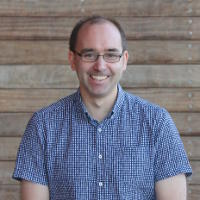
\includegraphics[width=1.0\textwidth]{dlj}
\end{column}
\end{columns}


\end{frame}
\note{
\setlength{\parskip}{0.5em}
}
 
%%%%%%%%%%%%%%%%%%%%%%%%%%%%%%%%%%%%%%%%%

\begin{frame}
\frametitle{Automation evangelist}
%\framesubtitle{}
\setlength{\parskip}{0.5em}

\begin{columns}[T]
\begin{column}[T]{0.7\textwidth}
\setlength{\parskip}{0.7em}
DevOps
\begin{enumerate}
\item From Software Engineering
\item Combining {\it Dev\/}elopment with {\it Op\/}erations
\item Promotes automation in software development, integration, testing, deployment and analytics
\end{enumerate}

Some of the same techniques can be used in research

\end{column}
\begin{column}[T]{0.3\textwidth}
\vspace{0.0em}
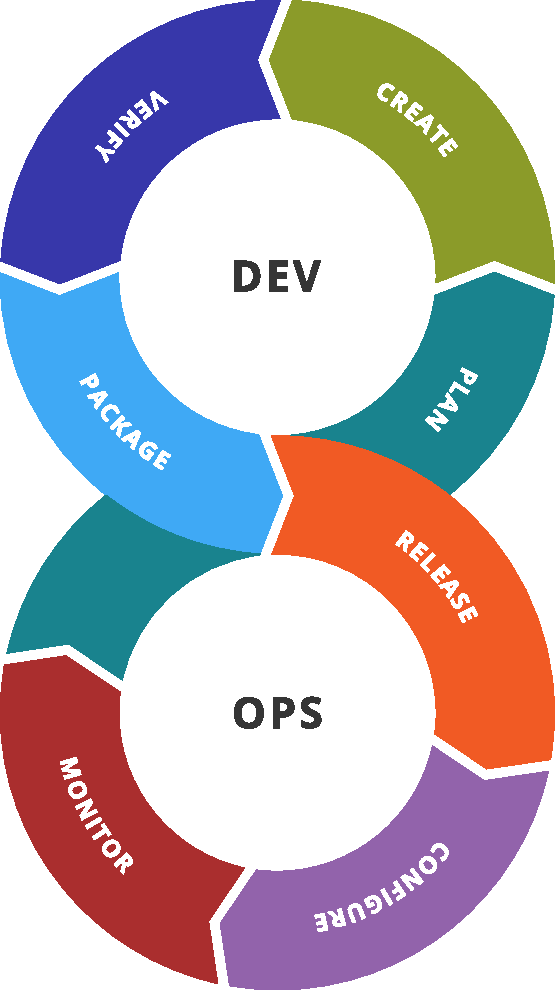
\includegraphics[width=1.0\textwidth]{devops}
\end{column}
\end{columns}


\end{frame}
\note{
\setlength{\parskip}{0.5em}
Setting the scene.
}
 
%%%%%%%%%%%%%%%%%%%%%%%%%%%%%%%%%%%%%%%%%

\begin{frame}
\frametitle{Is It Worth the Time?}
\framesubtitle{}
\setlength{\parskip}{0.5em}

{%

\centering
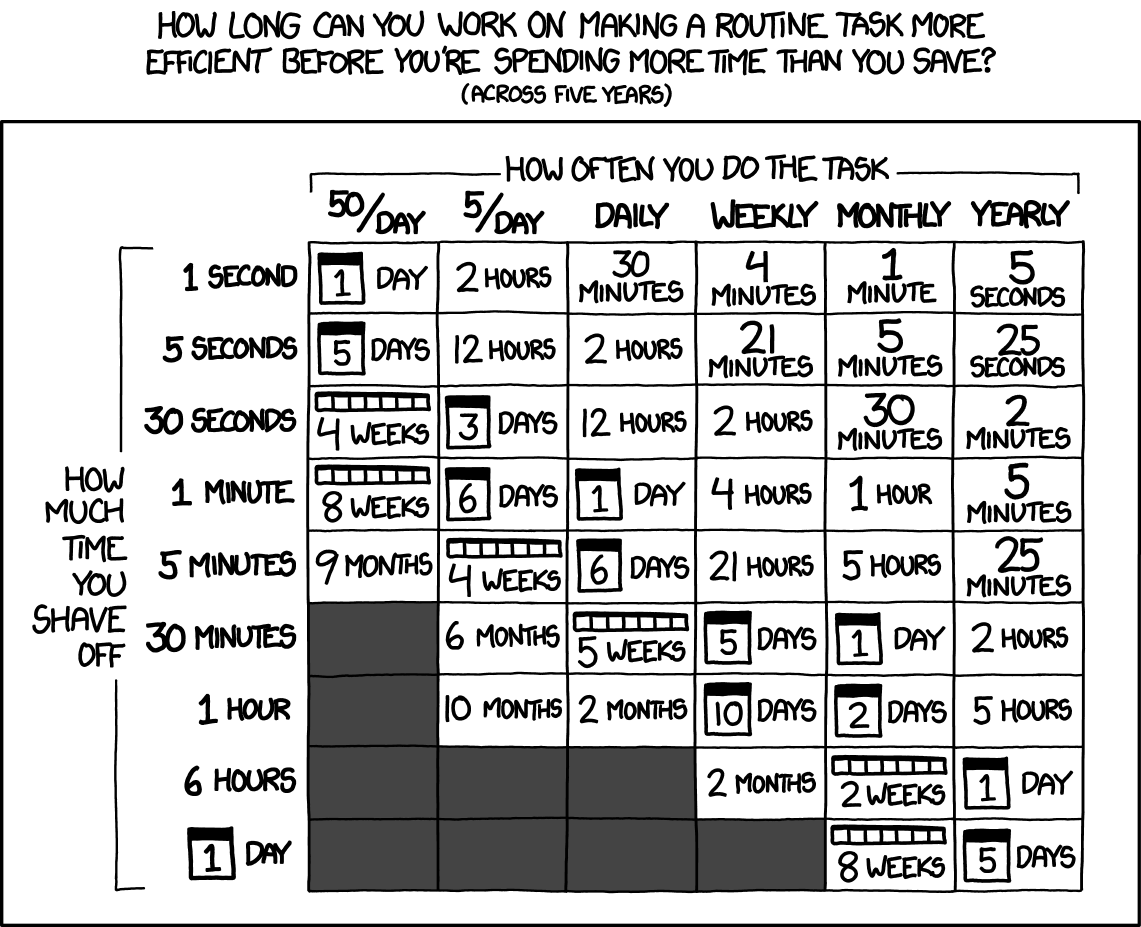
\includegraphics[width=0.7\textwidth]{xkcd-automation}

}%

{\tiny \url{https://xkcd.com/1205/}}

\end{frame}
\note{
\setlength{\parskip}{0.5em}
}

%%%%%%%%%%%%%%%%%%%%%%%%%%%%%%%%%%%%%%%%%

\begin{frame}
\frametitle{Data visualisation tools}
%\framesubtitle{}
\setlength{\parskip}{0.5em}

\begin{columns}[T]
\begin{column}[T]{0.45\textwidth}
\setlength{\parskip}{0.7em}
There are many tools

\begin{enumerate}
\item Excel
\item R/RGL
\item gnuplot
\item Matlab/Octave
\item Blender
\item Matplotlib
\end{enumerate}

All of these can be automated

\end{column}
\begin{column}[T]{0.55\textwidth}
\vspace{0.0em}
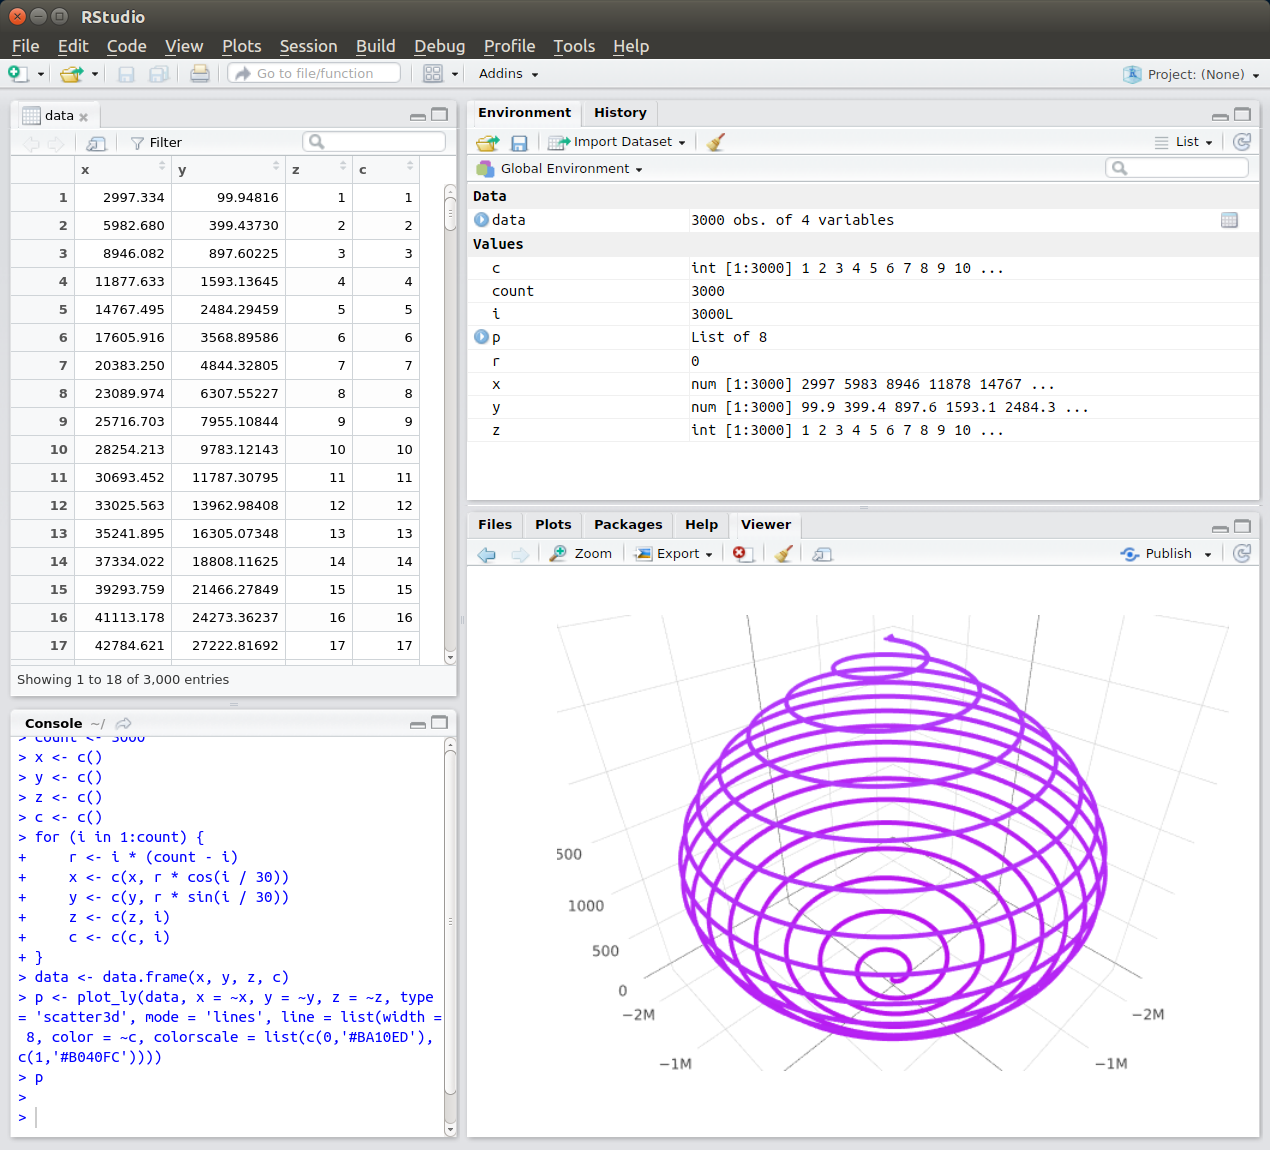
\includegraphics[width=1.0\textwidth]{rstudio}
\end{column}
\end{columns}


\end{frame}
\note{
\setlength{\parskip}{0.5em}
}
 
%%%%%%%%%%%%%%%%%%%%%%%%%%%%%%%%%%%%%%%%%

\begin{frame}[fragile]
\frametitle{Strange attractor -- generating data $(t, x, y, z)$}
%\framesubtitle{}
\setlength{\parskip}{0.5em}

\begin{columns}[T]
\begin{column}[T]{0.5\textwidth}
\setlength{\parskip}{0.7em}

% See https://github.com/olivierverdier/python-latex-highlighting
\begin{python}
import numpy as np
from scipy.integrate import odeint

rho = 28.0
sigma = 10.0
beta = 8.0 / 3.0

def f(state, t):
  x, y, z = state
  return \
    sigma * (y - x), \
    x * (rho - z) - y, \
    x * y - beta * z

state0 = [1.0, 1.0, 1.0]
t = np.arange(0.0, 40.0, 0.01)
states = odeint(f, state0, t)

data = np.column_stack((t, states))

np.savetxt("data.txt", data)






££  ££
\end{python}

\end{column}
\begin{column}[T]{0.5\textwidth}
%\vspace{-1.0em}

\begin{python}
0.000e+00 1.000e+00 1.000e+00 1.000e+00
1.000e-02 1.012e+00 1.259e+00 9.848e-01
2.000e-02 1.048e+00 1.524e+00 9.731e-01
2.999e-02 1.107e+00 1.798e+00 9.651e-01
4.000e-02 1.186e+00 2.088e+00 9.617e-01
5.000e-02 1.287e+00 2.400e+00 9.638e-01
5.999e-02 1.409e+00 2.738e+00 9.726e-01
7.000e-02 1.553e+00 3.109e+00 9.897e-01
8.000e-02 1.721e+00 3.517e+00 1.017e+00
8.999e-02 1.913e+00 3.969e+00 1.057e+00
1.000e-01 2.133e+00 4.471e+00 1.113e+00
1.100e-01 2.382e+00 5.029e+00 1.190e+00
1.199e-01 2.663e+00 5.650e+00 1.291e+00
1.300e-01 2.980e+00 6.341e+00 1.424e+00
1.400e-01 3.337e+00 7.110e+00 1.596e+00
1.499e-01 3.736e+00 7.964e+00 1.817e+00
1.600e-01 4.184e+00 8.910e+00 2.099e+00
1.700e-01 4.683e+00 9.955e+00 2.456e+00
1.799e-01 5.239e+00 1.110e+01 2.907e+00
1.900e-01 5.858e+00 1.236e+01 3.473e+00
2.000e-01 6.542e+00 1.373e+01 4.180e+00
2.099e-01 7.297e+00 1.520e+01 5.058e+00
2.200e-01 8.124e+00 1.677e+01 6.141e+00
2.300e-01 9.026e+00 1.841e+01 7.468e+00
2.399e-01 1.000e+01 2.009e+01 9.080e+00
2.500e-01 1.104e+01 2.177e+01 1.101e+01
2.600e-01 1.214e+01 2.338e+01 1.331e+01
2.700e-01 1.328e+01 2.484e+01 1.599e+01
\end{python}

\end{column}
\end{columns}


\end{frame}
\note{
\setlength{\parskip}{0.5em}
}
 
%%%%%%%%%%%%%%%%%%%%%%%%%%%%%%%%%%%%%%%%%

\begin{frame}[fragile]
\frametitle{R import and export}
%\framesubtitle{}
\setlength{\parskip}{0.5em}

\begin{columns}[T]
\begin{column}[T]{1.1\textwidth}
\vspace{-0.5em}

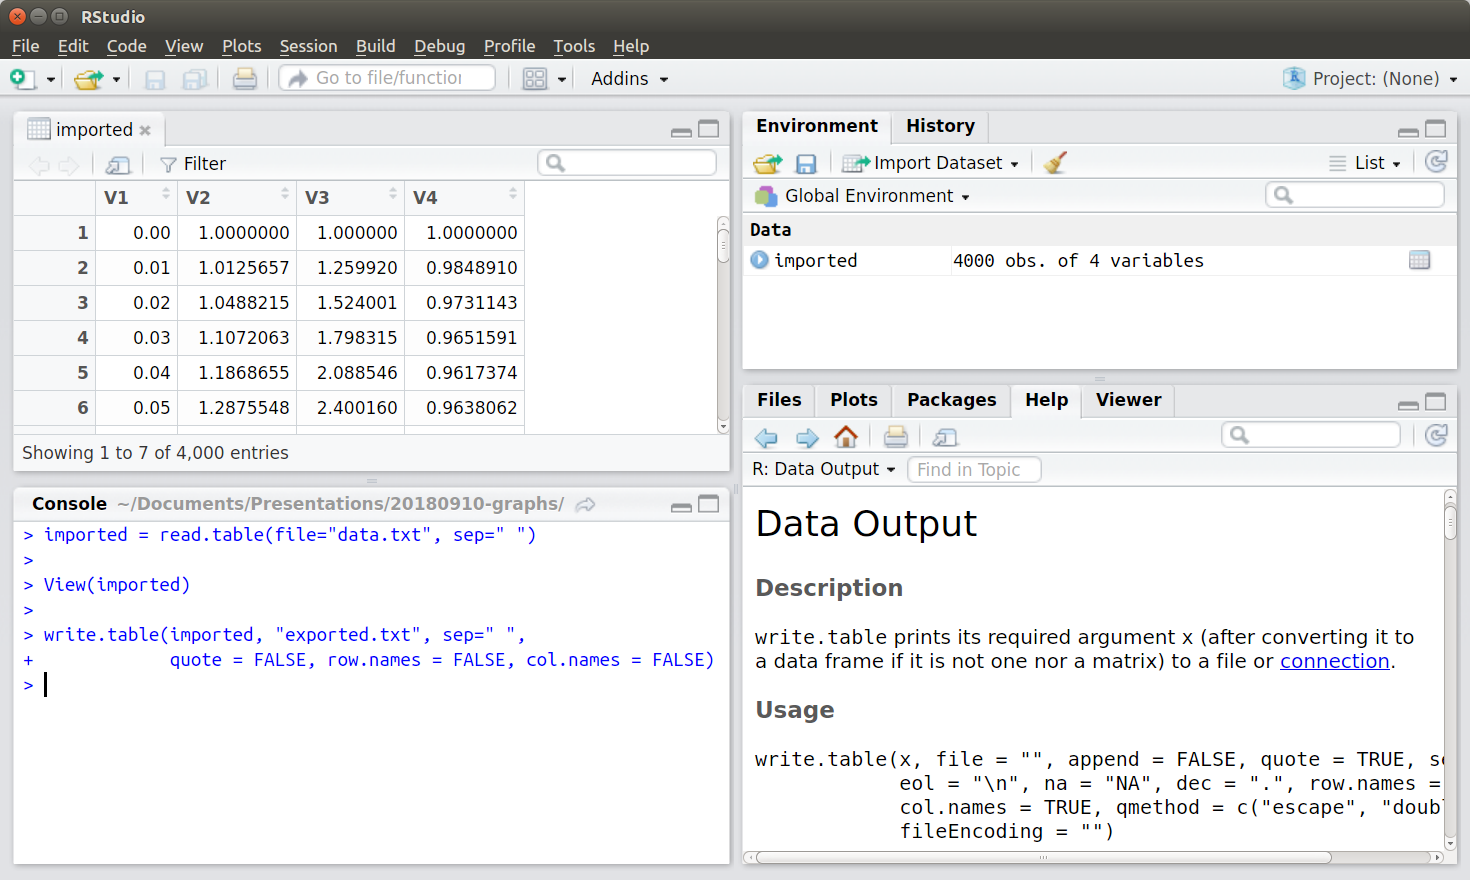
\includegraphics[width=1.0\textwidth]{rimportexport}

\end{column}
\end{columns}


\end{frame}
\note{
\setlength{\parskip}{0.5em}
}

%%%%%%%%%%%%%%%%%%%%%%%%%%%%%%%%%%%%%%%%%

\begin{frame}[fragile]
\frametitle{Rendering the data}
%\framesubtitle{}
\setlength{\parskip}{0.5em}

\begin{columns}[T]
\begin{column}[T]{0.5\textwidth}
\setlength{\parskip}{0.7em}

% See https://github.com/olivierverdier/python-latex-highlighting
\begin{python}
import numpy as np
import matplotlib.pyplot as plt


data = np.loadtxt("data.txt")

fig1 = plt.figure(figsize=(6.5, 8))

ax1 = fig1.gca()

ax1.set_title("Strange Attractor")
ax1.set_xlabel("Time")
ax1.set_ylabel("x position")


ax1.plot(data[:,0], data[:,1])



plt.savefig("fig.pdf", format="pdf")
plt.show()






££  ££
\end{python}

\end{column}
\begin{column}[T]{0.5\textwidth}
%\vspace{-1.0em}

\includegraphics[height=0.9\textheight]{strange01}
\end{column}
\end{columns}


\end{frame}
\note{
\setlength{\parskip}{0.5em}
}
 
%%%%%%%%%%%%%%%%%%%%%%%%%%%%%%%%%%%%%%%%%

\begin{frame}[fragile]
\frametitle{Overlaying graphs}
%\framesubtitle{}
\setlength{\parskip}{0.5em}

\begin{columns}[T]
\begin{column}[T]{0.5\textwidth}
\setlength{\parskip}{0.7em}

% See https://github.com/olivierverdier/python-latex-highlighting
\begin{python}
import numpy as np
import matplotlib.pyplot as plt


data = np.loadtxt("data.txt")

fig1 = plt.figure(figsize=(6.5, 8))

ax1 = fig1.gca()

ax1.set_title("Strange Attractor")
ax1.set_xlabel("Time")
ax1.set_ylabel("x position")


ax1.plot(data[:,0], data[:,1])
ax1.plot(data[:,0], data[:,2])
ax1.plot(data[:,0], data[:,3])

plt.savefig("fig.pdf", format="pdf")
plt.show()






££  ££
\end{python}

\end{column}
\begin{column}[T]{0.5\textwidth}
%\vspace{-1.0em}

\includegraphics[height=0.9\textheight]{strange02}
\end{column}
\end{columns}


\end{frame}
\note{
\setlength{\parskip}{0.5em}
}
 
%%%%%%%%%%%%%%%%%%%%%%%%%%%%%%%%%%%%%%%%%

\begin{frame}[fragile]
\frametitle{Three dimensional projection}
%\framesubtitle{}
\setlength{\parskip}{0.5em}

\begin{columns}[T]
\begin{column}[T]{0.5\textwidth}
\setlength{\parskip}{0.7em}

% See https://github.com/olivierverdier/python-latex-highlighting
\begin{python}
import numpy as np
import matplotlib.pyplot as plt
from mpl_toolkits.mplot3d import Axes3D

data = np.loadtxt("data.txt")

fig1 = plt.figure(figsize=(6.5, 8))

ax1 = fig1.gca(projection='3d')

ax1.set_title("Strange Attractor")
ax1.set_xlabel("x")
ax1.set_ylabel("y")
ax1.set_zlabel("z")

ax1.plot(data[:,1],data[:,2],data[:,3])



plt.savefig("fig.pdf", format="pdf")
plt.show()






££  ££
\end{python}

\end{column}
\begin{column}[T]{0.5\textwidth}
\vspace{2.5em}

\includegraphics[width=1.1\textwidth]{strange03}
\end{column}
\end{columns}


\end{frame}
\note{
\setlength{\parskip}{0.5em}
}

%%%%%%%%%%%%%%%%%%%%%%%%%%%%%%%%%%%%%%%%%

\begin{frame}[fragile]
\frametitle{Real example -- automarking}
%\framesubtitle{}
\setlength{\parskip}{0.5em}

\begin{columns}[T]
\begin{column}[T]{0.5\textwidth}
\setlength{\parskip}{0.7em}

\begin{enumerate}
\item Automatically mark programming coursework
\item Collect metrics from work submitted by students
\item Based on code quality and correct execution
\item Compare against marks assigned by real assessors
\item Use AI/optimisation to classify future work
\item Generate formative feedback for students
\end{enumerate}

\end{column}
\begin{column}[T]{0.5\textwidth}
\vspace{-0.5em}

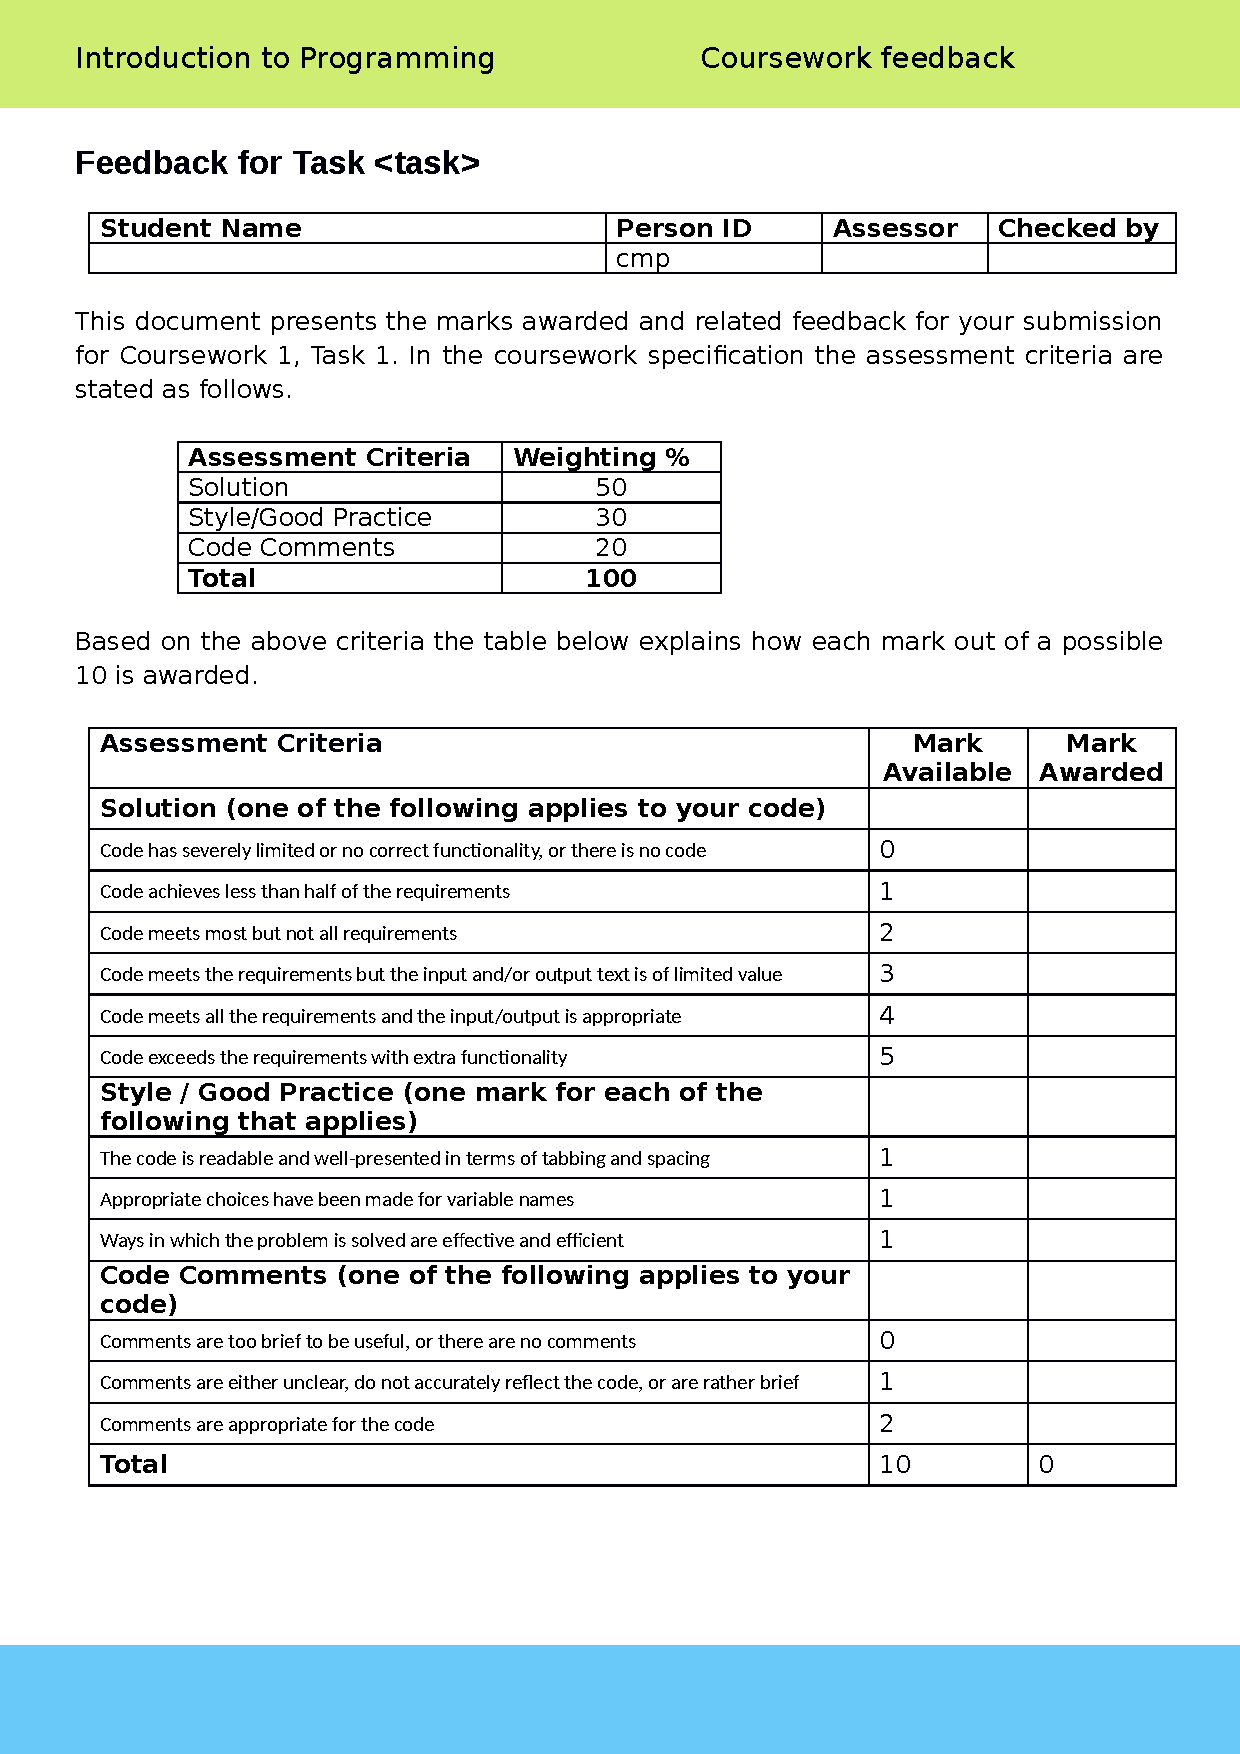
\includegraphics[width=1.0\textwidth]{feedback}
\end{column}
\end{columns}


\end{frame}
\note{
\setlength{\parskip}{0.5em}
}

%%%%%%%%%%%%%%%%%%%%%%%%%%%%%%%%%%%%%%%%%

\begin{frame}[fragile]
\frametitle{Automarking process}
%\framesubtitle{}
\setlength{\parskip}{0.5em}

\begin{columns}[T]
\begin{column}[T]{1.0\textwidth}
\vspace{-0.75em}

\includegraphics[width=1.0\textwidth]{automark-process}

\end{column}
\end{columns}


\end{frame}
\note{
\setlength{\parskip}{0.5em}
}

%%%%%%%%%%%%%%%%%%%%%%%%%%%%%%%%%%%%%%%%%

\begin{frame}[fragile]
\frametitle{Visualising the optimisation parameters}
%\framesubtitle{}
\setlength{\parskip}{0.5em}

\begin{columns}[T]
\begin{column}[T]{0.5\textwidth}
\setlength{\parskip}{0.7em}

% See https://github.com/olivierverdier/python-latex-highlighting
\begin{python}
import numpy as np
import matplotlib.pyplot as plt
from mpl_toolkits.mplot3d import Axes3D

data = np.loadtxt("data.txt")

x, y = np.meshgrid(np.arange(0,40,1), \
                   np.arange(0,40,1))

fig1 = plt.figure(figsize=(10, 8))

ax1 = fig1.gca(projection='3d')

ax1.set_title("Optimisation")
ax1.set_xlabel("Threshold $a$")
ax1.set_ylabel("Threshold $b$")
ax1.set_zlabel("Error")

ax1.plot_surface(x, y, data, \
  cstride=1, rstride=1, cmap='rainbow')

ax1.view_init(35, 15)

plt.savefig("fig.pdf", format="pdf")
plt.show()


££  ££
\end{python}

\end{column}
\begin{column}[T]{0.5\textwidth}
\vspace{2.5em}

\includegraphics[width=1.1\textwidth]{automark01}
\end{column}
\end{columns}


\end{frame}
\note{
\setlength{\parskip}{0.5em}
}

%%%%%%%%%%%%%%%%%%%%%%%%%%%%%%%%%%%%%%%%%

\begin{frame}[fragile]
\frametitle{Blender import}
%\framesubtitle{}
\setlength{\parskip}{0.5em}

\begin{columns}[T]
\begin{column}[T]{1.1\textwidth}
\vspace{-0.5em}

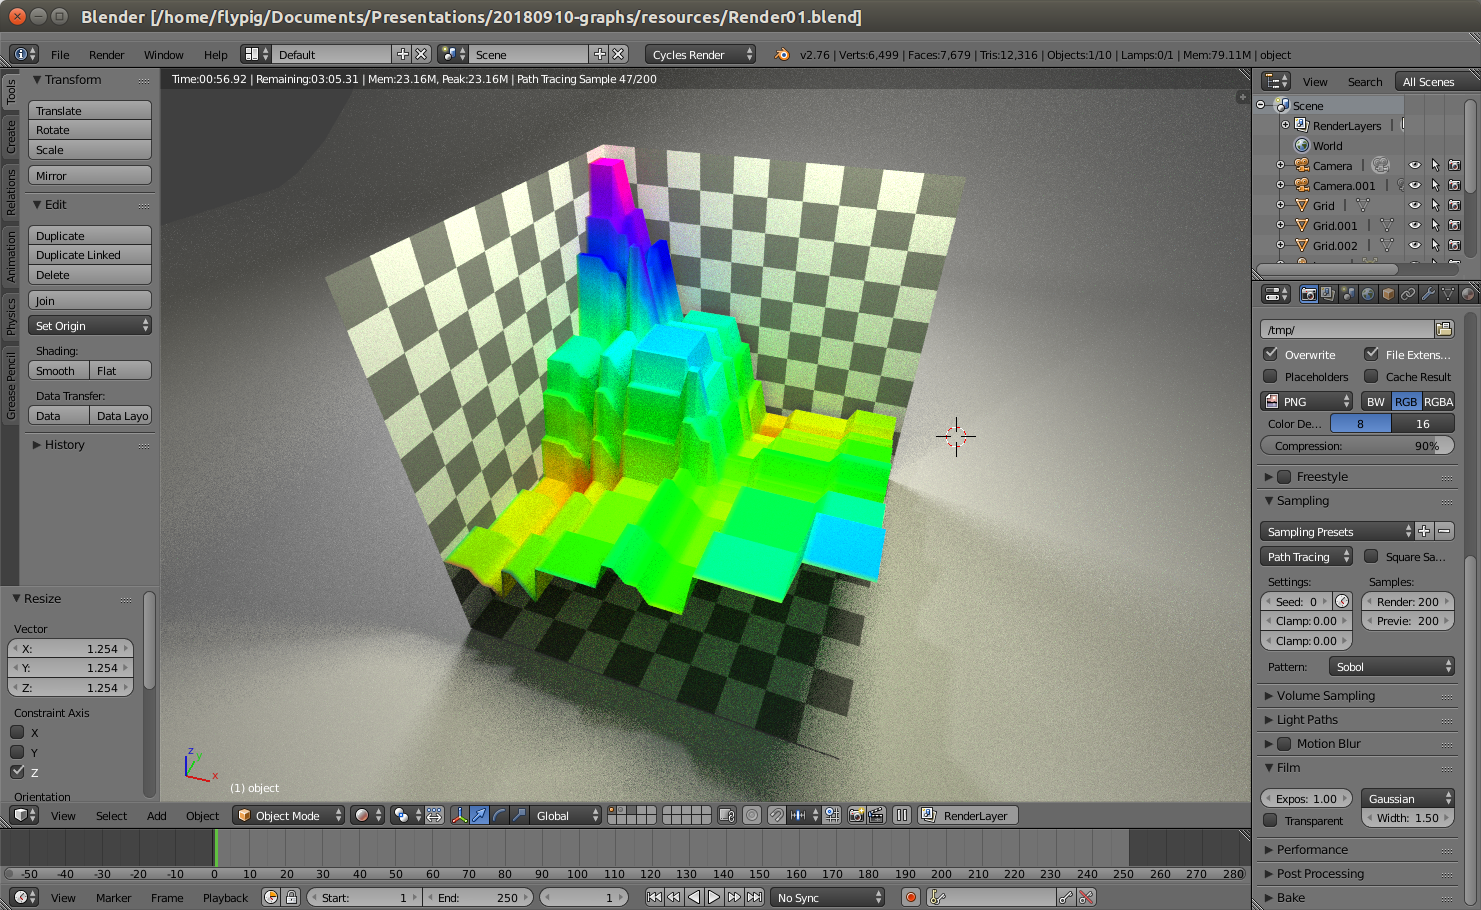
\includegraphics[width=1.0\textwidth]{blender}

\end{column}
\end{columns}


\end{frame}
\note{
\setlength{\parskip}{0.5em}
}
%%%%%%%%%%%%%%%%%%%%%%%%%%%%%%%%%%%%%%%%%

\begin{frame}[fragile]
\frametitle{Contact}
%\framesubtitle{}

\begin{columns}[T]
\begin{column}[T]{1.0\textwidth}
\setlength{\parskip}{1.0em}

Grab the scripts and code from Github: \\
\qquad \url{https://github.com/llewelld/graphgen-presentation}

Email: \\
\qquad \href{mailto:David.Llewellyn-Jones@cl.cam.ac.uk}{David.Llewellyn-Jones@cl.cam.ac.uk}

Website: \\
\qquad \url{http://www.flypig.co.uk}

\end{column}
\end{columns}


\end{frame}
\note{
\setlength{\parskip}{0.5em}
}

%%%%%%%%%%%%%%%%%%%%%%%%%%%%%%%%%%%%%%%%%

\end{document}
